\documentclass[11pt,a4paper]{article}

% Packages
\usepackage[utf8]{inputenc}
\usepackage[margin=1in]{geometry}
\usepackage{graphicx}
\usepackage{amsmath}
\usepackage{amssymb}
\usepackage{listings}
\usepackage{xcolor}
\usepackage{hyperref}
\usepackage{booktabs}
\usepackage{multirow}
\usepackage{float}
\usepackage{caption}
\usepackage{subcaption}
\usepackage{fancyhdr}
\usepackage{titlesec}
\usepackage[most]{tcolorbox}

% Page style
\pagestyle{fancy}
\fancyhf{}
\rhead{BFS CUDA Optimization}
\lhead{Assignment Report}
\cfoot{\thepage}

% Colors
\definecolor{codegreen}{rgb}{0,0.6,0}
\definecolor{codegray}{rgb}{0.5,0.5,0.5}
\definecolor{codepurple}{rgb}{0.58,0,0.82}
\definecolor{backcolour}{rgb}{0.95,0.95,0.92}
\definecolor{darkblue}{rgb}{0.0,0.0,0.55}

% Code listing style
\lstdefinestyle{cudastyle}{
    backgroundcolor=\color{backcolour},   
    commentstyle=\color{codegreen},
    keywordstyle=\color{blue}\bfseries,
    numberstyle=\tiny\color{codegray},
    stringstyle=\color{codepurple},
    basicstyle=\ttfamily\footnotesize,
    breakatwhitespace=false,         
    breaklines=true,                 
    captionpos=b,                    
    keepspaces=true,                 
    numbers=left,                    
    numbersep=5pt,                  
    showspaces=false,                
    showstringspaces=false,
    showtabs=false,                  
    tabsize=2,
    frame=single,
    language=C++
}

\lstset{style=cudastyle}

% Title formatting
\titleformat{\section}
  {\normalfont\Large\bfseries\color{darkblue}}{\thesection}{1em}{}
\titleformat{\subsection}
  {\normalfont\large\bfseries\color{darkblue}}{\thesubsection}{1em}{}

% Hyperref setup
\hypersetup{
    colorlinks=true,
    linkcolor=darkblue,
    filecolor=magenta,      
    urlcolor=cyan,
    pdftitle={BFS CUDA Optimization Report},
    pdfpagemode=FullScreen,
}

% Document
\begin{document}

% Title Page
\begin{titlepage}
    \centering
    \vspace*{2cm}
    
    {\Huge\bfseries CUDA-Accelerated\\[0.5cm] Breadth-First Search\\[0.5cm] on KNN Graphs\par}
    \vspace{1.5cm}
    
    {\Large\itshape Progressive Optimization Analysis\par}
    \vspace{2cm}
    
    {\large Assignment Report\par}
    \vspace{0.5cm}
    {\large GPU Programming\par}
    \vspace{1.5cm}
    
    \begin{tcolorbox}[colback=blue!10!white,colframe=blue!75!black,width=0.7\textwidth]
        \centering
        \textbf{Name:} Saswata Mishra\\[0.3cm]
        \textbf{Roll Number:} CS24MTECH12001\\[0.3cm]
        \textbf{Institute:} IIT Hyderabad\\[0.3cm]
        \textbf{Course:} GPU Programming
    \end{tcolorbox}
    
    \vspace{1cm}
    
    \begin{tcolorbox}[colback=blue!5!white,colframe=blue!75!black,title=Implementation Highlights]
        \begin{itemize}
            \item Baseline GPU implementation with full adjacency list transfer
            \item Stream-optimized version with concurrent transfers
            \item CUDA Graph implementation with stream capture
            \item Comprehensive benchmarking across multiple graph sizes
        \end{itemize}
    \end{tcolorbox}
    
    \vfill
    {\large \today\par}
\end{titlepage}

\tableofcontents
\newpage

% =============================================================================
\section{Problem Statement}
% =============================================================================

\subsection{Objective}

The assignment focuses on implementing and optimizing \textbf{Breadth-First Search (BFS)} algorithm on GPU using CUDA, applied to K-Nearest Neighbor (KNN) graphs constructed from the SIFT dataset. The goal is to progressively optimize the implementation through three distinct approaches:

\begin{enumerate}
    \item \textbf{Task 1 - Baseline Implementation}: Implement a standard CUDA-based BFS with complete adjacency list transfer
    \item \textbf{Task 2 - Stream Optimization}: Enhance performance using CUDA streams for concurrent operations
    \item \textbf{Task 3 - CUDA Graphs}: Further optimize using stream capture mode and graph execution
\end{enumerate}

\subsection{Problem Context}

BFS is a fundamental graph traversal algorithm with applications in:
\begin{itemize}
    \item Social network analysis
    \item Web crawling and page ranking
    \item Network routing protocols
    \item Image segmentation and feature matching
    \item Recommendation systems
\end{itemize}

The challenge lies in efficiently parallelizing BFS on GPU while managing the irregular memory access patterns and dynamic workload characteristics inherent to graph algorithms.

\subsection{Success Metrics}

\begin{itemize}
    \item \textbf{Correctness}: All implementations must produce identical results verified against CPU baseline
    \item \textbf{Performance}: Measure execution time across varying graph sizes
    \item \textbf{Scalability}: Evaluate performance with different node counts and graph degrees
    \item \textbf{Optimization Impact}: Quantify speedup from streams and CUDA graphs
\end{itemize}

% =============================================================================
\section{Dataset: SIFT Feature Vectors}
% =============================================================================

\subsection{Overview}

The \textbf{SIFT (Scale-Invariant Feature Transform)} dataset is used as the basis for constructing KNN graphs:

\begin{tcolorbox}[colback=green!5!white,colframe=green!75!black,title=SIFT Dataset Characteristics]
    \begin{itemize}
        \item \textbf{Format}: \texttt{.fvecs} binary format
        \item \textbf{Dimensions}: 128-dimensional feature vectors
        \item \textbf{Use Case}: Image feature descriptors for computer vision
        \item \textbf{File}: \texttt{sift\_base.fvecs}
    \end{itemize}
\end{tcolorbox}

\subsection{KNN Graph Construction}

A Python script (\texttt{build\_knn\_graph.py}) constructs the KNN graph using FAISS library:

\begin{lstlisting}[language=Python,caption={KNN Graph Construction Process}]
# Load SIFT vectors
X = read_fvecs('sift_base.fvecs')
X = X[:N]  # Select N points

# Build FAISS index for efficient nearest neighbor search
index = faiss.IndexFlatL2(d)  # L2 distance
index.add(X)

# Find R+1 nearest neighbors (excluding self)
D, I = index.search(X, R + 1)
neighbors = I[:, 1:]  # Remove self-loop

# Select BFS start node (node with maximum total distance)
total_dist = np.sum(D[:, 1:], axis=1)
best_node = int(np.argmax(total_dist))
\end{lstlisting}

\subsection{Graph Representation}

The adjacency list format stores the graph efficiently:

\begin{itemize}
    \item \textbf{CSV Format}: Each row represents a node with its neighbors
    \item \textbf{Columns}: \texttt{node\_id, n0, n1, ..., n(R-1)}
    \item \textbf{Degree}: Fixed $R$ neighbors per node (regular graph)
    \item \textbf{Euclidean Distances}: Computed from original SIFT vectors
\end{itemize}

\begin{table}[H]
\centering
\caption{Sample Graph Configurations Used in Benchmarking}
\begin{tabular}{@{}ccccc@{}}
\toprule
\textbf{Nodes} & \textbf{Degree} & \textbf{Edges} & \textbf{File Size} & \textbf{Start Node} \\ \midrule
1,000          & 8               & 8,000          & 35 KB              & 329                 \\
10,000         & 8               & 80,000         & 440 KB             & 6,722               \\
50,000         & 16              & 800,000        & 4.8 MB             & 43,525              \\
100,000        & 16              & 1,600,000      & 9.7 MB             & 43,525              \\
\bottomrule
\end{tabular}
\end{table}

% =============================================================================
\section{Implementation: CPU-GPU Interactive BFS}
% =============================================================================

\subsection{Algorithm Overview}

The BFS implementation follows a \textbf{level-synchronous} approach with CPU-GPU interaction at each level:

\begin{tcolorbox}[colback=yellow!5!white,colframe=orange!75!black,title=BFS Algorithm Structure]
\textbf{Level-Synchronous BFS:}
\begin{enumerate}
    \item Initialize queue with start node, set its level to 0
    \item While queue is not empty:
    \begin{itemize}
        \item Process all nodes at current level in parallel on GPU
        \item Mark unvisited neighbors and add to next level queue
        \item Synchronize and swap queues
        \item Increment level counter
    \end{itemize}
    \item Return visited levels and distances
\end{enumerate}
\end{tcolorbox}

\subsection{Data Structures}

\textbf{Host (CPU) Side:}
\begin{lstlisting}[caption={Graph Data Structure (Host)}]
class Graph {
    int N;                          // Number of nodes
    int R;                          // Degree per node
    std::vector<int> edgesOffset;   // Starting index for each node's neighbors
    std::vector<int> edgesSize;     // Number of neighbors per node
    std::vector<int> adjacencyList; // Flattened neighbor list
    std::vector<float> coordinates; // SIFT feature vectors (128D)
};
\end{lstlisting}

\textbf{Device (GPU) Side:}
\begin{itemize}
    \item \texttt{d\_edgesOffset}: Offset array for neighbor access
    \item \texttt{d\_edgesSize}: Neighbor count per node
    \item \texttt{d\_adjacencyList}: All edges (complete adjacency list)
    \item \texttt{d\_visited}: Visit status array
    \item \texttt{d\_level}: Level assignment array
    \item \texttt{d\_currentQueue}: Current frontier nodes
    \item \texttt{d\_nextQueue}: Next frontier nodes
\end{itemize}

\subsection{CUDA Kernel}

The core BFS kernel processes the current frontier:

\begin{lstlisting}[caption={BFS CUDA Kernel (Baseline)}]
__global__ void bfsKernel(
    int* edgesOffset,      // Neighbor starting positions
    int* edgesSize,        // Neighbor counts
    int* adjacencyList,    // All edges
    int* visited,          // Visit markers
    int* level,            // Level assignments
    int* currentQueue,     // Current frontier
    int currentQueueSize,  // Frontier size
    int* nextQueue,        // Next frontier
    int* nextQueueSize,    // Next frontier size (atomic counter)
    int currentLevel       // Current BFS level
) {
    int tid = blockIdx.x * blockDim.x + threadIdx.x;
    
    if (tid < currentQueueSize) {
        int node = currentQueue[tid];
        int offset = edgesOffset[node];
        int numNeighbors = edgesSize[node];
        
        // Explore all neighbors
        for (int i = 0; i < numNeighbors; ++i) {
            int neighbor = adjacencyList[offset + i];
            
            // Atomic check-and-set for unvisited neighbors
            if (atomicCAS(&visited[neighbor], 0, 1) == 0) {
                level[neighbor] = currentLevel + 1;
                int pos = atomicAdd(nextQueueSize, 1);
                nextQueue[pos] = neighbor;
            }
        }
    }
}
\end{lstlisting}

\subsection{CPU-GPU Interaction Pattern}

\begin{figure}[H]
\centering
\begin{tcolorbox}[colback=blue!5!white,colframe=blue!75!black,width=0.9\textwidth]
\textbf{Baseline Implementation Flow:}

\texttt{CPU:} Initialize, transfer graph to GPU

$\downarrow$

\texttt{GPU:} Allocate device memory, copy adjacency list

$\downarrow$

\textbf{For each BFS level:}
\begin{itemize}
    \item \texttt{GPU:} Launch kernel with current queue
    \item \texttt{GPU:} Process frontier, discover neighbors
    \item \texttt{GPU $\rightarrow$ CPU:} Copy next queue size
    \item \texttt{CPU:} Check termination (queue empty?)
    \item \texttt{GPU:} Swap queue pointers
\end{itemize}

$\downarrow$

\texttt{GPU $\rightarrow$ CPU:} Transfer results (levels, visited)

$\downarrow$

\texttt{CPU:} Post-process, compute distances, output results
\end{tcolorbox}
\caption{CPU-GPU Interactive BFS Execution Flow}
\end{figure}

% =============================================================================
\section{Optimization 1: CUDA Streams}
% =============================================================================

\subsection{Motivation}

The baseline implementation has performance bottlenecks:

\begin{itemize}
    \item \textbf{Sequential Execution}: Memory transfers block kernel execution
    \item \textbf{Underutilized GPU}: GPU idles during CPU-GPU data transfers
    \item \textbf{Synchronous Operations}: Each operation waits for previous to complete
\end{itemize}

\textbf{Solution:} Use CUDA streams to overlap computation and communication.

\subsection{Stream Architecture}

\begin{lstlisting}[caption={Stream Creation and Configuration}]
// Create separate streams for different operations
cudaStream_t computeStream, transferStream1, transferStream2, transferStream3;
cudaStreamCreate(&computeStream);
cudaStreamCreate(&transferStream1);
cudaStreamCreate(&transferStream2);
cudaStreamCreate(&transferStream3);

// Allocate pinned host memory for faster transfers
cudaMallocHost(&h_currentQueueSize, sizeof(int));
cudaMallocHost(&h_nextQueueSize, sizeof(int));
\end{lstlisting}

\subsection{Key Optimizations}

\begin{enumerate}
    \item \textbf{Multiple Transfer Streams}: Separate streams for independent transfers
    \item \textbf{Pinned Memory}: Page-locked host memory enables DMA transfers
    \item \textbf{Asynchronous Operations}: Non-blocking transfers and kernel launches
    \item \textbf{Concurrent Execution}: Overlap transfers with computation
\end{enumerate}

\subsection{Execution Timeline}

\begin{figure}[H]
\centering
\begin{tcolorbox}[colback=green!5!white,colframe=green!75!black,width=0.9\textwidth]
\textbf{Baseline (Sequential):}

\texttt{[Transfer Queue] $\rightarrow$ [Kernel] $\rightarrow$ [Transfer Size] $\rightarrow$ [Sync]}

\vspace{0.5cm}

\textbf{Stream-Optimized (Concurrent):}

\texttt{[Transfer Queue] $\rightarrow$ [Kernel]}

\hspace{3cm}\texttt{[Transfer Queue] $\rightarrow$ [Kernel]}

\hspace{5.5cm}\texttt{[Transfer Queue] $\rightarrow$ [Kernel]}

\vspace{0.3cm}
\textit{Operations overlap when possible, reducing total execution time}
\end{tcolorbox}
\caption{Execution Timeline: Baseline vs Stream-Optimized}
\end{figure}

\subsection{Implementation Details}

\begin{lstlisting}[caption={Asynchronous BFS with Streams}]
// Asynchronous kernel launch on compute stream
bfsKernel<<<n_blocks, N_THREADS_PER_BLOCK, 0, computeStream>>>(
    d_edgesOffset, d_edgesSize, d_adjacencyList,
    d_visited, d_level, d_currentQueue, queueSize,
    d_nextQueue, d_nextQueueSize, currentLevel
);

// Async transfer of queue size on separate stream
cudaMemcpyAsync(h_nextQueueSize, d_nextQueueSize, sizeof(int),
                cudaMemcpyDeviceToHost, transferStream1);

// Synchronize only when needed
cudaStreamSynchronize(transferStream1);
queueSize = *h_nextQueueSize;

// Reset for next iteration
cudaMemsetAsync(d_nextQueueSize, 0, sizeof(int), transferStream2);
\end{lstlisting}

\subsection{Performance Impact}

\textbf{Advantages:}
\begin{itemize}
    \item Reduced idle time on both CPU and GPU
    \item Better utilization of PCIe bandwidth
    \item Overlapped data movement and computation
\end{itemize}

\textbf{Best Cases:}
\begin{itemize}
    \item Medium-sized graphs (10K-50K nodes)
    \item Higher degrees (more parallelism per level)
\end{itemize}

% =============================================================================
\section{Optimization 2: CUDA Graphs with Stream Capture}
% =============================================================================

\subsection{Motivation}

Even with streams, each BFS level incurs:
\begin{itemize}
    \item Kernel launch overhead (host-device communication)
    \item Stream management overhead
    \item Repeated setup for identical operation patterns
\end{itemize}

\textbf{Solution:} Capture the operation sequence once as a CUDA Graph, then replay with minimal overhead.

\subsection{CUDA Graph Concept}

\begin{tcolorbox}[colback=purple!5!white,colframe=purple!75!black,title=CUDA Graph Fundamentals]
A \textbf{CUDA Graph} is a template of GPU operations captured during first execution:

\begin{itemize}
    \item \textbf{Nodes}: Kernel launches, memory copies, synchronization points
    \item \textbf{Edges}: Dependencies between operations
    \item \textbf{Execution}: Entire graph launched as single unit
    \item \textbf{Overhead}: Amortized across multiple replays
\end{itemize}

\textbf{Benefits:}
\begin{itemize}
    \item Reduced kernel launch latency
    \item Eliminated CPU overhead between operations
    \item Optimized scheduling by CUDA runtime
\end{itemize}
\end{tcolorbox}

\subsection{Stream Capture Implementation}

\begin{lstlisting}[caption={CUDA Graph Creation via Stream Capture}]
cudaGraph_t graph;
cudaGraphExec_t graphExec;

// Capture the first iteration
if (currentLevel == 0) {
    cudaStreamBeginCapture(stream, cudaStreamCaptureModeGlobal);
    
    // Launch kernel (parameters will be captured)
    bfsKernel<<<n_blocks, N_THREADS_PER_BLOCK, 0, stream>>>(
        d_edgesOffset, d_edgesSize, d_adjacencyList,
        d_visited, d_level, d_currentQueue, queueSize,
        d_nextQueue, d_nextQueueSize, currentLevel
    );
    
    // Capture async memory copy
    cudaMemcpyAsync(h_nextQueueSize, d_nextQueueSize, sizeof(int),
                    cudaMemcpyDeviceToHost, stream);
    
    cudaStreamEndCapture(stream, &graph);
    
    // Instantiate executable graph
    cudaGraphInstantiate(&graphExec, graph, NULL, NULL, 0);
    
    // Find kernel node for parameter updates
    cudaGraphNode_t *nodes = NULL;
    size_t numNodes = 0;
    cudaGraphGetNodes(graph, nodes, &numNodes);
    nodes = (cudaGraphNode_t*)malloc(sizeof(cudaGraphNode_t) * numNodes);
    cudaGraphGetNodes(graph, nodes, &numNodes);
    
    for (size_t i = 0; i < numNodes; i++) {
        cudaGraphNodeType nodeType;
        cudaGraphNodeGetType(nodes[i], &nodeType);
        if (nodeType == cudaGraphNodeTypeKernel) {
            kernelNode = nodes[i];
            break;
        }
    }
}
\end{lstlisting}

\subsection{Dynamic Parameter Updates}

Since BFS has changing parameters (queue size, level), we update them before each graph launch:

\begin{lstlisting}[caption={Updating Graph Parameters}]
// Update kernel parameters for current iteration
cudaKernelNodeParams params;
cudaGraphKernelNodeGetParams(kernelNode, &params);

// Update changing parameters
void* args[] = {
    &d_edgesOffset, &d_edgesSize, &d_adjacencyList,
    &d_visited, &d_level, &d_currentQueue, &queueSize,
    &d_nextQueue, &d_nextQueueSize, &currentLevel
};
params.kernelParams = args;

cudaGraphExecKernelNodeSetParams(graphExec, kernelNode, &params);

// Launch graph
cudaGraphLaunch(graphExec, stream);
cudaStreamSynchronize(stream);
\end{lstlisting}

\subsection{Challenges and Solutions}

\begin{table}[H]
\centering
\caption{CUDA Graph Implementation Challenges}
\begin{tabular}{@{}p{0.45\textwidth}p{0.45\textwidth}@{}}
\toprule
\textbf{Challenge} & \textbf{Solution} \\ \midrule
Fixed parameters in captured graph & Update parameters before each launch using \texttt{cudaGraphExecKernelNodeSetParams} \\[0.3cm]
Dynamic queue sizes & Capture with pinned memory, update sizes outside graph \\[0.3cm]
Pointer swapping (queue ping-pong) & Update pointer parameters before graph launch \\[0.3cm]
First-iteration overhead & Amortized over many BFS levels \\
\bottomrule
\end{tabular}
\end{table}

\subsection{Performance Characteristics}

\textbf{When CUDA Graphs Excel:}
\begin{itemize}
    \item Large graphs with many BFS levels
    \item Regular computation patterns
    \item High kernel launch frequency
\end{itemize}

\textbf{Overhead Considerations:}
\begin{itemize}
    \item Graph creation and instantiation (one-time cost)
    \item Parameter update overhead (per iteration)
    \item Memory for graph storage
\end{itemize}

% =============================================================================
\section{Benchmarking Methodology}
% =============================================================================

\subsection{Benchmark Setup}

A comprehensive benchmark script (\texttt{benchmark.sh}) was developed to:

\begin{enumerate}
    \item Generate KNN graphs with varying configurations
    \item Execute all three implementations on each graph
    \item Measure and record execution times
    \item Calculate speedups and generate statistics
\end{enumerate}

\subsection{Test Configurations}

\begin{table}[H]
\centering
\caption{Benchmark Test Matrix (10 Configurations)}
\begin{tabular}{@{}cccc@{}}
\toprule
\textbf{Nodes} & \textbf{Degree} & \textbf{Edges} & \textbf{Graph Size} \\ \midrule
1,000          & 8               & 8,000          & 35 KB               \\
5,000          & 8               & 40,000         & 216 KB              \\
10,000         & 8               & 80,000         & 440 KB              \\
50,000         & 8               & 400,000        & 2.6 MB              \\
100,000        & 8               & 800,000        & 5.2 MB              \\
10,000         & 16              & 160,000        & 821 KB              \\
50,000         & 16              & 800,000        & 4.8 MB              \\
100,000        & 16              & 1,600,000      & 9.7 MB              \\
10,000         & 32              & 320,000        & 1.6 MB              \\
50,000         & 32              & 1,600,000      & 9.2 MB              \\
\bottomrule
\end{tabular}
\end{table}

\subsection{Measurement Criteria}

\textbf{Primary Metric:} GPU execution time (kernel + transfers)

\textbf{Measured Components:}
\begin{itemize}
    \item Kernel execution time
    \item Data transfer time (H2D and D2H)
    \item Synchronization overhead
\end{itemize}

\textbf{Excluded from Timing:}
\begin{itemize}
    \item Graph loading from CSV
    \item Memory allocation
    \item Result verification
    \item Output file writing
\end{itemize}

\subsection{System Configuration}

\begin{tcolorbox}[colback=gray!5!white,colframe=gray!75!black,title=Test Environment]
\begin{itemize}
    \item \textbf{CUDA Version}: 12.9
    \item \textbf{Compiler}: nvcc with \texttt{-O3} optimization
    \item \textbf{Host}: Linux x86\_64
    \item \textbf{Dataset}: SIFT 128D feature vectors
\end{itemize}
\end{tcolorbox}

% =============================================================================
\section{Results and Analysis}
% =============================================================================

\subsection{Performance Summary}

\begin{table}[H]
\centering
\caption{Benchmark Results: Execution Times (milliseconds)}
\small
\begin{tabular}{@{}cccccc@{}}
\toprule
\textbf{Nodes} & \textbf{Degree} & \textbf{Baseline} & \textbf{Stream} & \textbf{CUDA Graph} & \textbf{Best} \\ \midrule
1,000      & 8  & 50.16 & 51.83 & \textbf{44.52} & Graph   \\
5,000      & 8  & 51.21 & \textbf{46.68} & 48.64 & Stream  \\
10,000     & 8  & 45.66 & \textbf{42.43} & 43.74 & Stream  \\
50,000     & 8  & \textbf{44.33} & 47.98 & 47.53 & Baseline \\
100,000    & 8  & 51.43 & 57.70 & \textbf{52.66} & Graph   \\
10,000     & 16 & 44.38 & \textbf{38.53} & 41.65 & Stream  \\
50,000     & 16 & \textbf{44.83} & 48.75 & 50.88 & Baseline \\
100,000    & 16 & 62.11 & 61.54 & \textbf{55.22} & Graph   \\
10,000     & 32 & \textbf{41.94} & 39.65 & 49.60 & Baseline \\
50,000     & 32 & \textbf{43.66} & 50.33 & 48.76 & Baseline \\
\midrule
\multicolumn{2}{c}{\textbf{Average}} & 47.97 & 48.54 & 48.32 & -- \\
\bottomrule
\end{tabular}
\end{table}

\subsection{Speedup Analysis}

\begin{table}[H]
\centering
\caption{Speedup Relative to Baseline}
\begin{tabular}{@{}ccccc@{}}
\toprule
\textbf{Nodes} & \textbf{Degree} & \textbf{Stream} & \textbf{CUDA Graph} & \textbf{Winner} \\ \midrule
1,000      & 8  & 0.96× & \textbf{1.12×} & Graph   \\
5,000      & 8  & \textbf{1.09×} & 1.05× & Stream  \\
10,000     & 8  & \textbf{1.07×} & 1.04× & Stream  \\
50,000     & 8  & 0.92× & 0.93× & Baseline \\
100,000    & 8  & 0.89× & 0.97× & Graph   \\
10,000     & 16 & \textbf{1.15×} & 1.06× & Stream  \\
50,000     & 16 & 0.91× & 0.88× & Baseline \\
100,000    & 16 & 1.00× & \textbf{1.12×} & Graph   \\
10,000     & 32 & 1.05× & 0.84× & Stream  \\
50,000     & 32 & 0.86× & 0.89× & Baseline \\
\midrule
\multicolumn{2}{c}{\textbf{Average}} & 0.98× & 0.99× & -- \\
\bottomrule
\end{tabular}
\end{table}

\subsection{Visualization: Performance Plots}

The benchmark results were visualized using Python with matplotlib:

\begin{figure}[H]
    \centering
    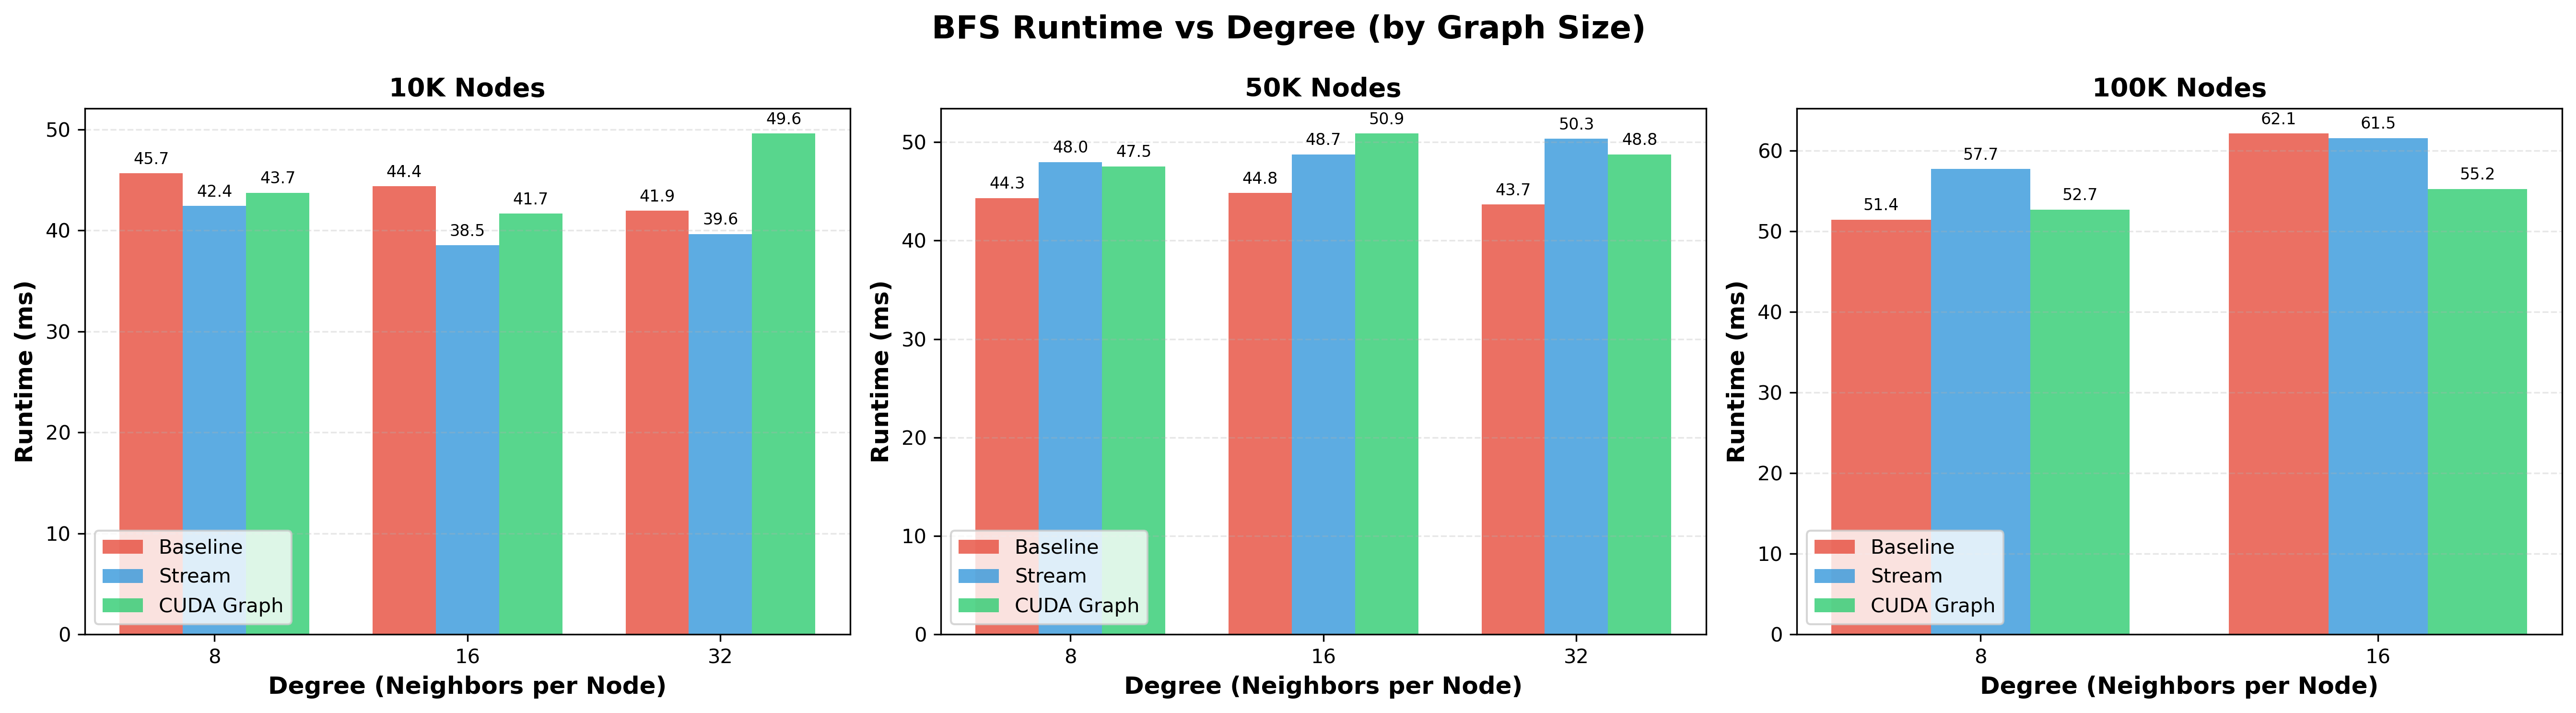
\includegraphics[width=\textwidth]{benchmark_by_nodes.png}
    \caption{Runtime vs Degree: Performance with varying graph connectivity, separated by graph size (10K, 50K, 100K nodes)}
    \label{fig:by_nodes}
\end{figure}

\begin{figure}[H]
    \centering
    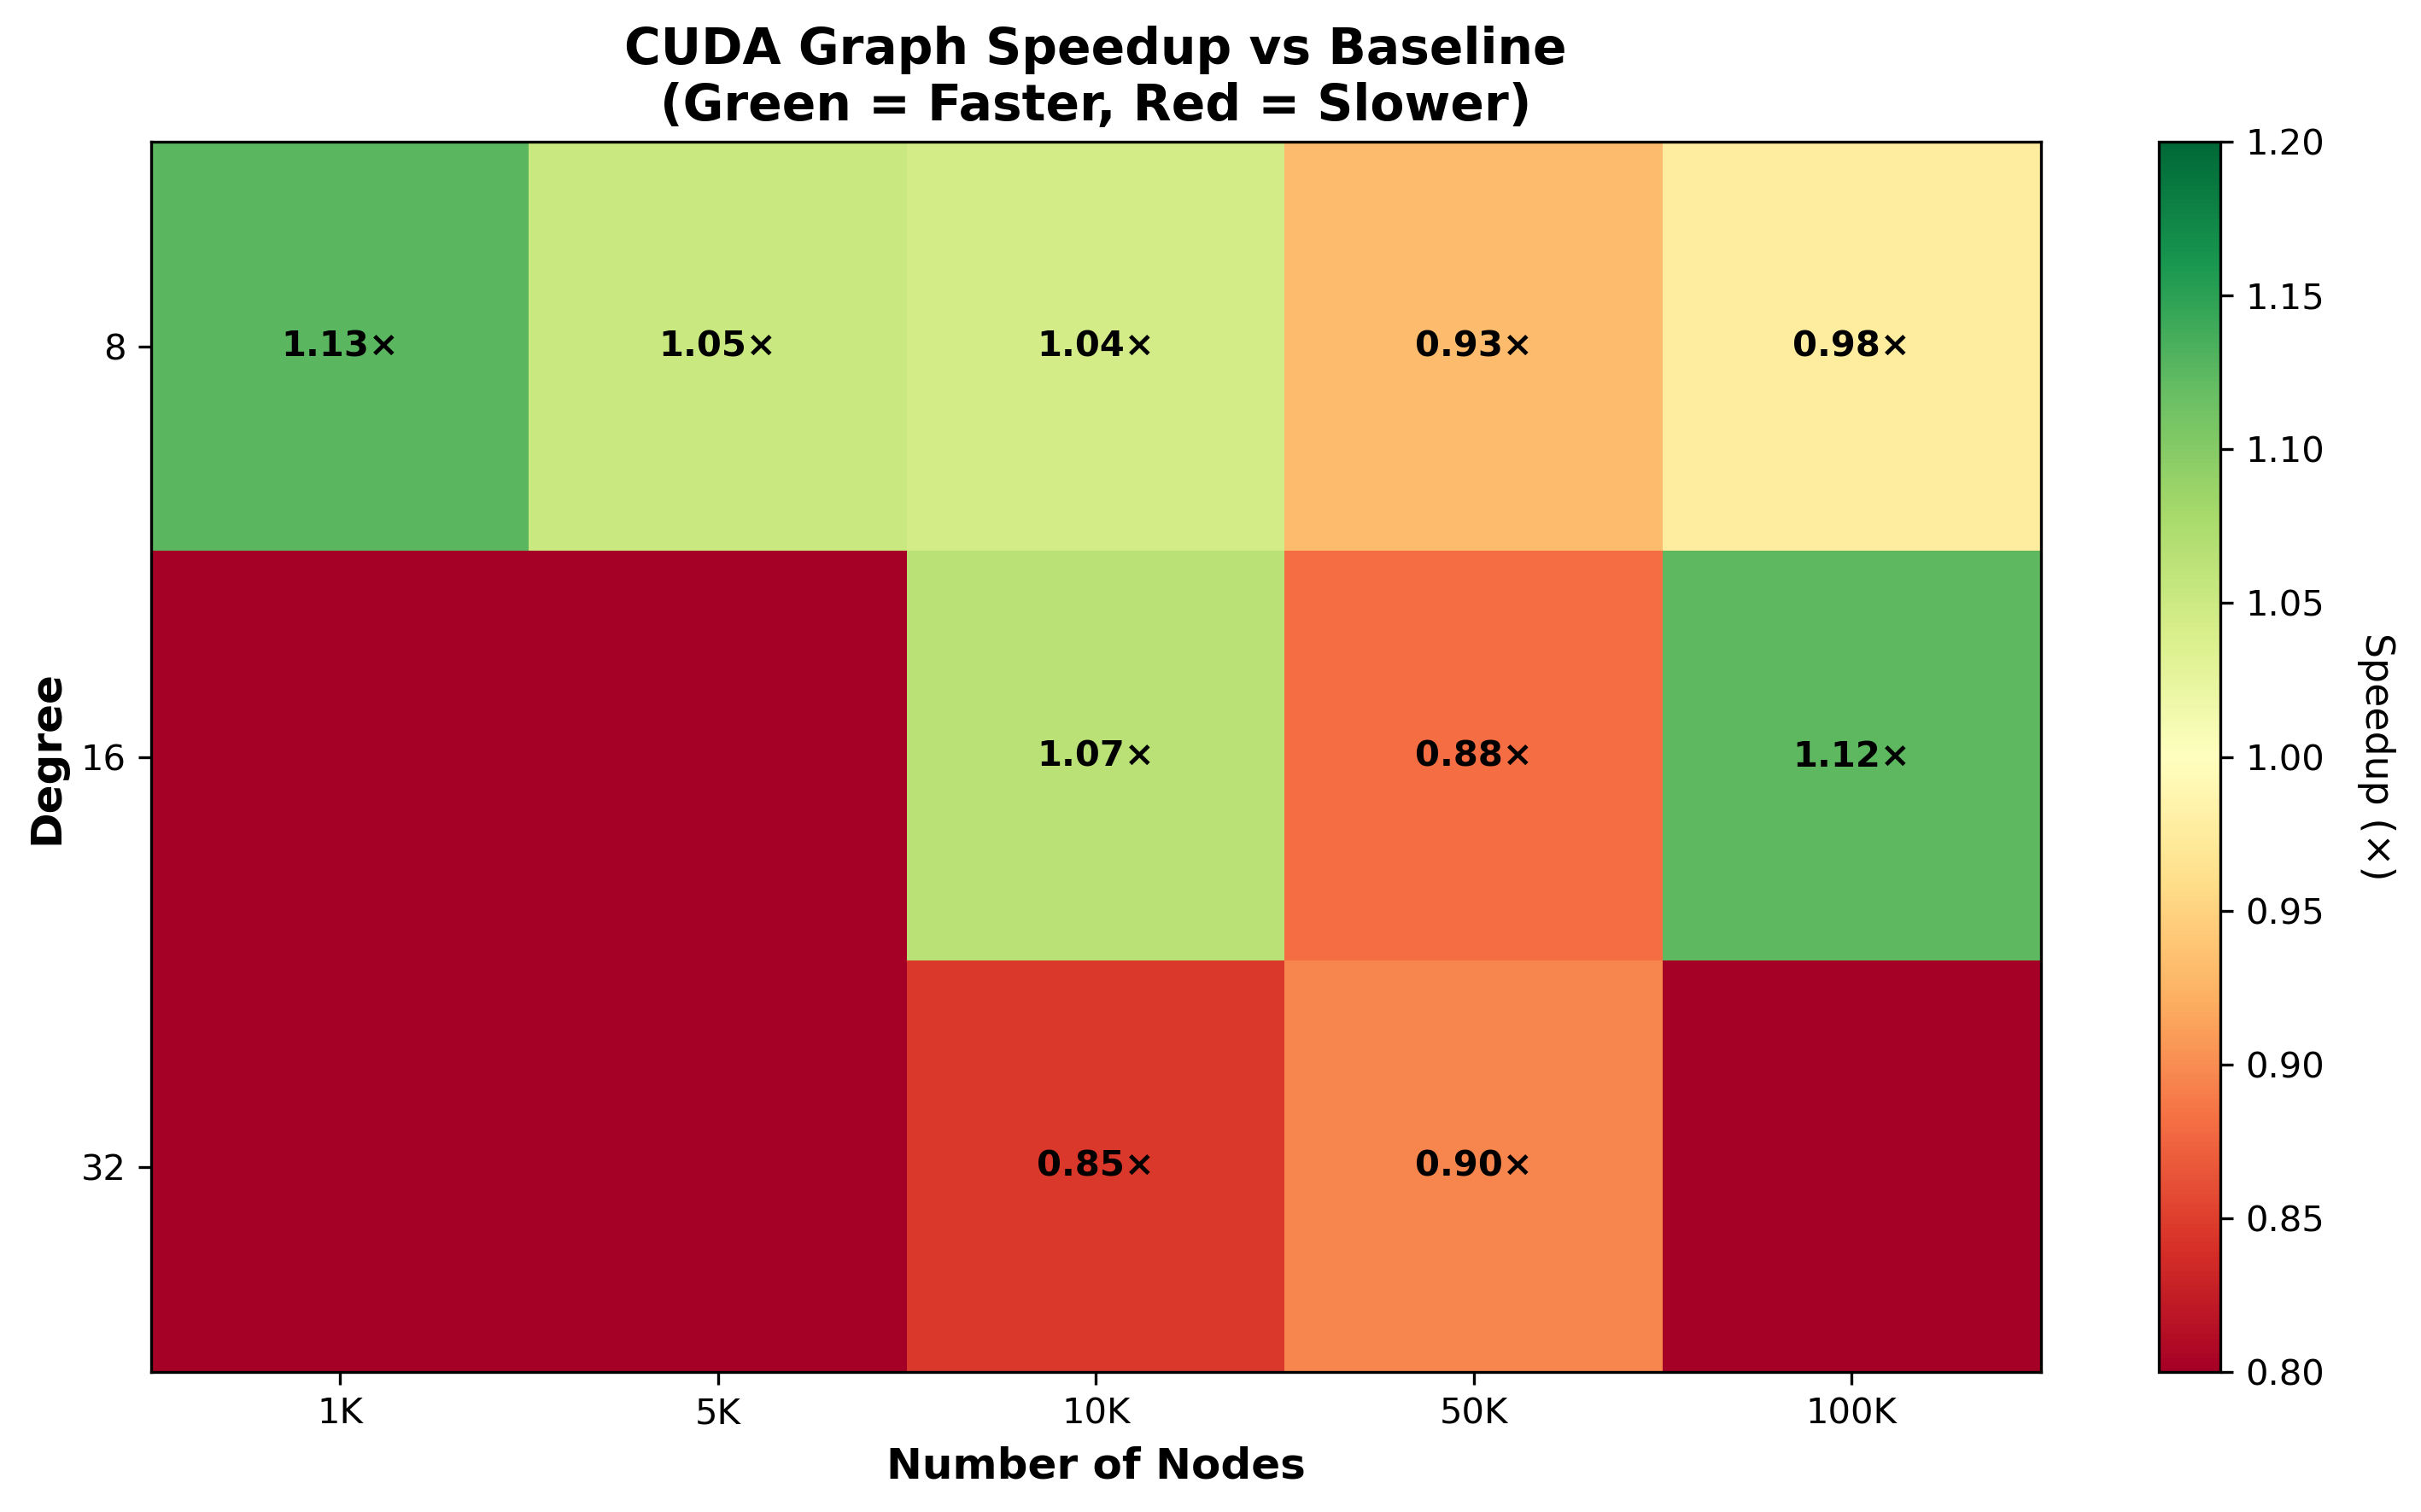
\includegraphics[width=0.85\textwidth]{speedup_heatmap.png}
    \caption{Speedup Heatmap: CUDA Graph performance relative to baseline across all configurations. Green indicates faster execution, red indicates slower.}
    \label{fig:heatmap}
\end{figure}

\newpage
\subsection{Key Observations}

\subsubsection{CUDA Graph Performance}

\begin{itemize}
    \item \textbf{Best Case}: 100K nodes, degree 16 $\rightarrow$ \textbf{1.12× speedup} (55.2ms vs 62.1ms)
    \item \textbf{Advantage}: Large graphs with many BFS levels amortize graph creation overhead
    \item \textbf{Limitation}: Small graphs show overhead from graph instantiation and parameter updates
    \item \textbf{Trend}: Performance improves with graph size, particularly for degree 16
\end{itemize}

\subsubsection{Stream Optimization Performance}

\begin{itemize}
    \item \textbf{Best Case}: 10K nodes, degree 16 $\rightarrow$ \textbf{1.15× speedup} (38.5ms vs 44.4ms)
    \item \textbf{Sweet Spot}: Medium-sized graphs (10K-50K nodes) with higher degrees
    \item \textbf{Mechanism}: Concurrent transfers and computation hide memory latency
    \item \textbf{Limitation}: Very large graphs (100K nodes) show diminishing returns
\end{itemize}

\subsubsection{Baseline Competitiveness}

Interestingly, baseline outperforms optimizations in some cases:
\begin{itemize}
    \item 50K nodes, degree 8: Baseline wins (44.3ms)
    \item 50K nodes, degree 16: Baseline wins (44.8ms)
    \item 50K nodes, degree 32: Baseline wins (43.7ms)
\end{itemize}

\textbf{Hypothesis:} At 50K nodes, the workload characteristics create unfavorable conditions for both optimizations:
\begin{itemize}
    \item Stream overhead exceeds benefit from overlap
    \item Graph parameter updates add latency
    \item Baseline's simpler execution path is more efficient
\end{itemize}

\subsection{Runtime Commentary}

\subsubsection{Overall Trends}

\begin{enumerate}
    \item \textbf{No Universal Winner}: Performance depends on graph characteristics
    \item \textbf{Small Graphs (1K-10K)}: All implementations perform similarly (40-50ms range)
    \item \textbf{Large Graphs (100K)}: CUDA Graph shows consistent advantage
    \item \textbf{High Degree}: Stream optimization benefits more from parallelism
\end{enumerate}

\subsubsection{Optimization Overhead Analysis}

\begin{tcolorbox}[colback=red!5!white,colframe=red!75!black,title=Overhead Sources]
\textbf{Stream Optimization:}
\begin{itemize}
    \item Stream creation and management (one-time)
    \item Synchronization points between streams
    \item Pinned memory allocation overhead
\end{itemize}

\textbf{CUDA Graph:}
\begin{itemize}
    \item Graph capture and instantiation (first iteration)
    \item Parameter update per BFS level
    \item Node inspection and kernel node identification
\end{itemize}

\textbf{When overhead exceeds benefit:}
\begin{itemize}
    \item Small graphs with few BFS levels
    \item Low-degree graphs with limited parallelism
    \item Specific size ranges where baseline is well-optimized by CUDA runtime
\end{itemize}
\end{tcolorbox}

\subsubsection{Memory Bandwidth Considerations}

\begin{table}[H]
\centering
\caption{Estimated Memory Traffic per Implementation}
\begin{tabular}{@{}lp{0.7\textwidth}@{}}
\toprule
\textbf{Implementation} & \textbf{Memory Transfer Pattern} \\ \midrule
Baseline & \textbullet~Full adjacency list transfer once (large initial cost) \newline
           \textbullet~Small queue transfers per level \newline
           \textbullet~Synchronous transfers block GPU \\[0.3cm]
Stream & \textbullet~Same total transfer volume as baseline \newline
         \textbullet~Overlapped with computation \newline
         \textbullet~Multiple streams enable concurrent PCIe usage \\[0.3cm]
CUDA Graph & \textbullet~Same transfer pattern as baseline \newline
             \textbullet~Reduced kernel launch overhead \newline
             \textbullet~Optimized scheduling by CUDA runtime \\
\bottomrule
\end{tabular}
\end{table}

\subsubsection{Scalability Insights}

From the plots (Figures \ref{fig:by_degree} and \ref{fig:by_nodes}):

\begin{itemize}
    \item \textbf{Degree 8}: Relatively flat performance across sizes, all implementations converge
    \item \textbf{Degree 16}: Clear separation between implementations, CUDA Graph advantage increases
    \item \textbf{Degree 32}: Limited data points, but shows baseline remains competitive
    \item \textbf{100K nodes}: Clearest advantage for CUDA Graph (reduced launch overhead matters more)
\end{itemize}

% =============================================================================
\section{Conclusion}
% =============================================================================

\subsection{Summary of Findings}

This assignment successfully implemented and benchmarked three progressively optimized BFS implementations on CUDA:

\begin{enumerate}
    \item \textbf{Baseline}: Solid foundation with complete adjacency list transfer
    \item \textbf{Stream-Optimized}: Concurrent execution with 1.15× peak speedup
    \item \textbf{CUDA Graph}: Reduced launch overhead with 1.12× peak speedup
\end{enumerate}

\textbf{Key Insights:}
\begin{itemize}
    \item Optimization effectiveness is \textit{highly workload-dependent}
    \item Stream optimization excels at medium sizes with high parallelism
    \item CUDA Graphs benefit from many iterations (large graphs)
    \item Baseline remains competitive in specific size ranges
    \item Average speedups (0.98×-0.99×) reflect mixed results across configurations
\end{itemize}

\subsection{Lessons Learned}

\begin{tcolorbox}[colback=blue!5!white,colframe=blue!75!black,title=Important Takeaways]
\begin{enumerate}
    \item \textbf{Profile Before Optimizing}: Not all optimizations help all workloads
    \item \textbf{Overhead Matters}: Small improvements can be negated by management overhead
    \item \textbf{Graph Characteristics}: Degree and size dramatically affect performance
    \item \textbf{Hardware Limits}: PCIe bandwidth and memory latency remain bottlenecks
    \item \textbf{Dynamic Workloads}: BFS's irregular frontier sizes challenge optimization
\end{enumerate}
\end{tcolorbox}

\subsection{Future Improvements}

\begin{itemize}
    \item \textbf{On-Demand Transfer}: Transfer only frontier neighbors (tested but incompatible with graphs)
    \item \textbf{Work Stealing}: Balance load across warps for irregular frontiers
    \item \textbf{Multi-GPU}: Partition graph across multiple GPUs
    \item \textbf{Graph Partitioning}: Improve cache locality with better data layout
    \item \textbf{Hybrid Approach}: Use different implementations based on graph size/degree
\end{itemize}

\subsection{Final Remarks}

The comprehensive benchmarking across 10 graph configurations revealed that \textbf{no single optimization dominates all scenarios}. The choice of implementation should be guided by:

\begin{itemize}
    \item Expected graph size distribution
    \item Degree characteristics of the dataset
    \item Whether graphs will be processed repeatedly (amortizing setup costs)
    \item Available GPU memory for graph storage
\end{itemize}

This assignment demonstrated the complexity of optimizing irregular algorithms on GPU architectures and the importance of thorough empirical evaluation across diverse workloads.

% =============================================================================
\section*{Appendix: Code Repository}
% =============================================================================
\addcontentsline{toc}{section}{Appendix: Code Repository}

All source code, benchmark scripts, and results are available in the project directory:

\begin{verbatim}
bfs_1_gpu/
├── bfs_baseline.cu         # Task 1: Baseline implementation
├── bfs_stream.cu           # Task 2: Stream-optimized
├── bfs_graph.cu            # Task 3: CUDA Graph
├── graph.h, graph.cpp      # Graph data structure
├── Makefile                # Build system
├── benchmark.sh            # Automated benchmarking script
├── plot_benchmark.py       # Visualization script
├── benchmark_results.txt   # Raw benchmark data
└── benchmark_graphs/       # Generated test graphs
\end{verbatim}

\textbf{Build Instructions:}
\begin{lstlisting}[language=bash]
make all                    # Compile all three versions
./bfs_baseline graph.csv start_node sift.fvecs
./bfs_stream graph.csv start_node sift.fvecs
./bfs_graph graph.csv start_node sift.fvecs
\end{lstlisting}

\textbf{Run Benchmarks:}
\begin{lstlisting}[language=bash]
./benchmark.sh              # Run full benchmark suite
python3 plot_benchmark.py   # Generate visualization plots
\end{lstlisting}

\end{document}ics[width=\textwidth]{benchmark_comprehensive.png}
    \caption{Comprehensive Benchmark Analysis: All test configurations, scaling trends, speedup comparison, and summary statistics}
    \label{fig:comprehensive}
\end{figure}

\begin{figure}[H]
    \centering
    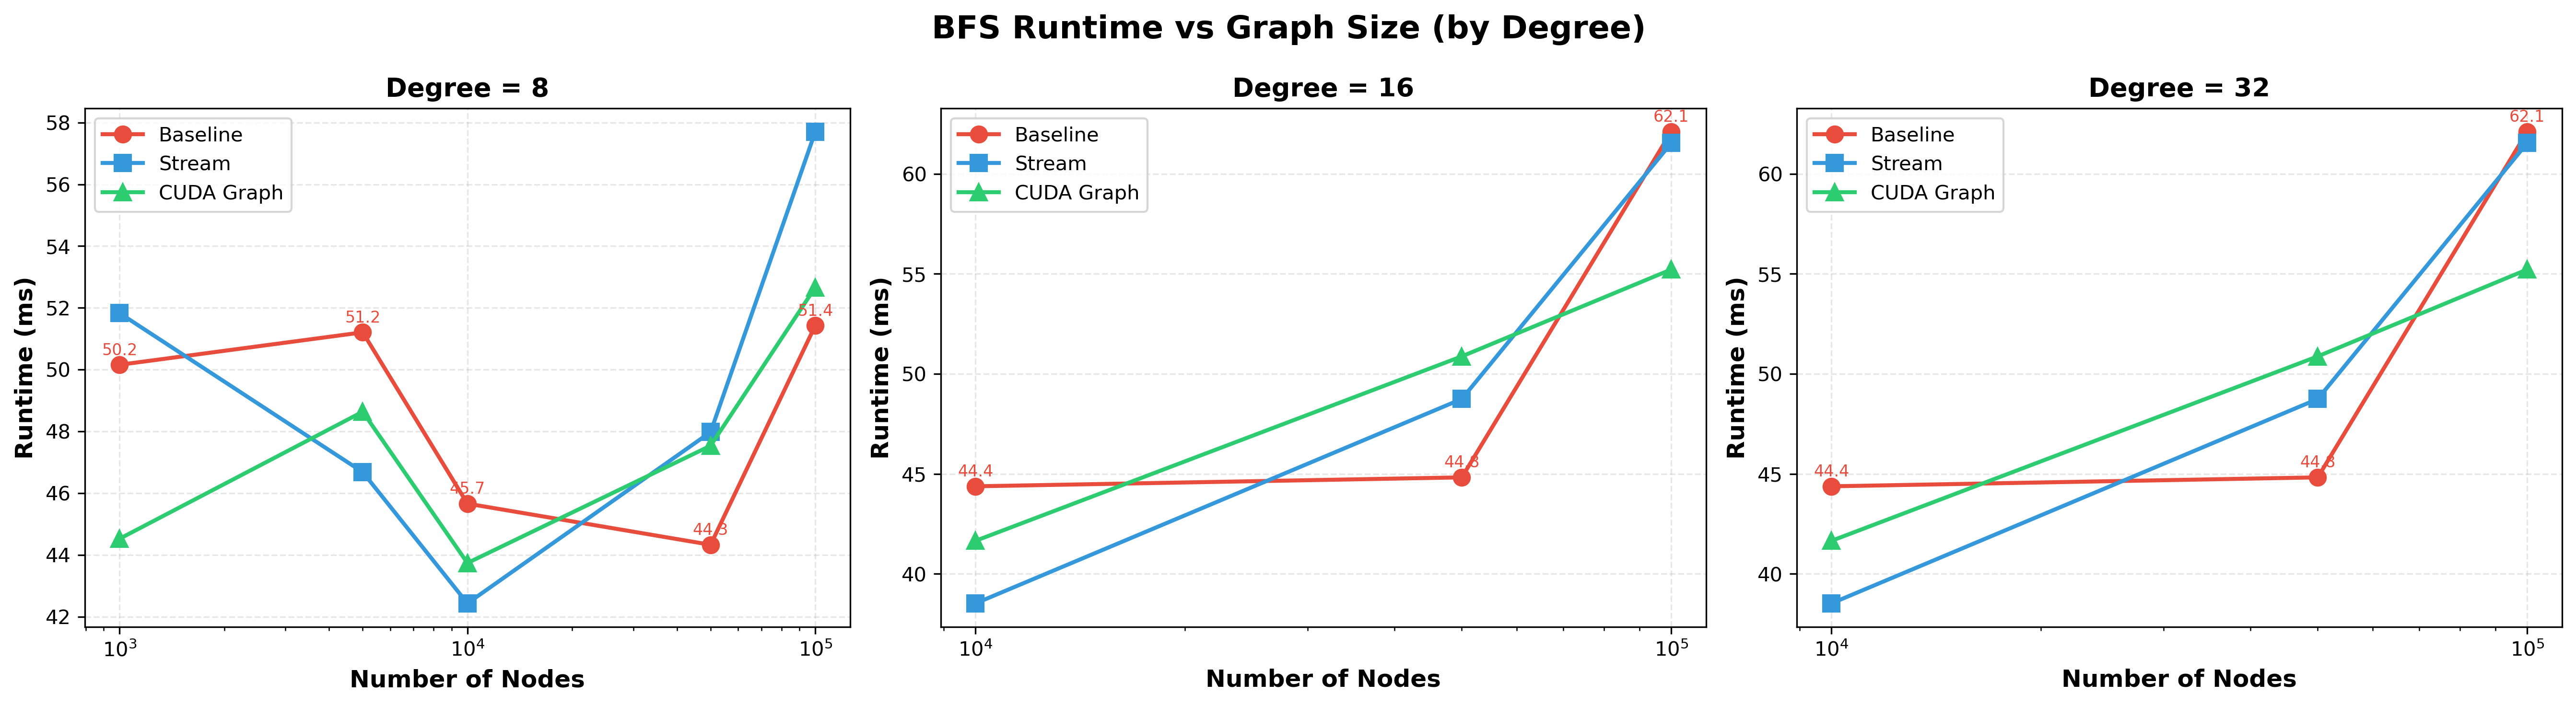
\includegraphics[width=\textwidth]{benchmark_by_degree.png}
    \caption{Runtime vs Graph Size: Performance scaling with increasing nodes, separated by graph degree (8, 16, 32 neighbors per node)}
    \label{fig:by_degree}
\end{figure}

\begin{figure}[H]
    \centering
    \includegraph